\chapter{OFDM radar signal processing}
\label{chap_OFDM}

Orthogonal frequency division modulation has been adopted in the current generation of wireless communication systems and will be adopted for 6G as well.
OFDM splits the wireless signal into multiple subcarriers, each modulated by a data stream. Multi carrier transmission offers numerous advantages such as high spectral efficiency and robustness to multipath fading. These factors make OFDM the ideal candidate for current and next generation high bit-rate applications and it's currently used in 5G and in IEEE 802.11 (WiFi).



\section{Structure of OFDM signal}

OFDM modulation efficiently distributes the signal over a discrete-time and discrete-frequency matrix. Each OFDM subcarrier is shaped using a rectangular window in the time domain, resulting in cardinal-sine-shaped carriers in the frequency domain \cite{Schaich_Wild_2014}.

\begin{figure}[H]
    \centering
    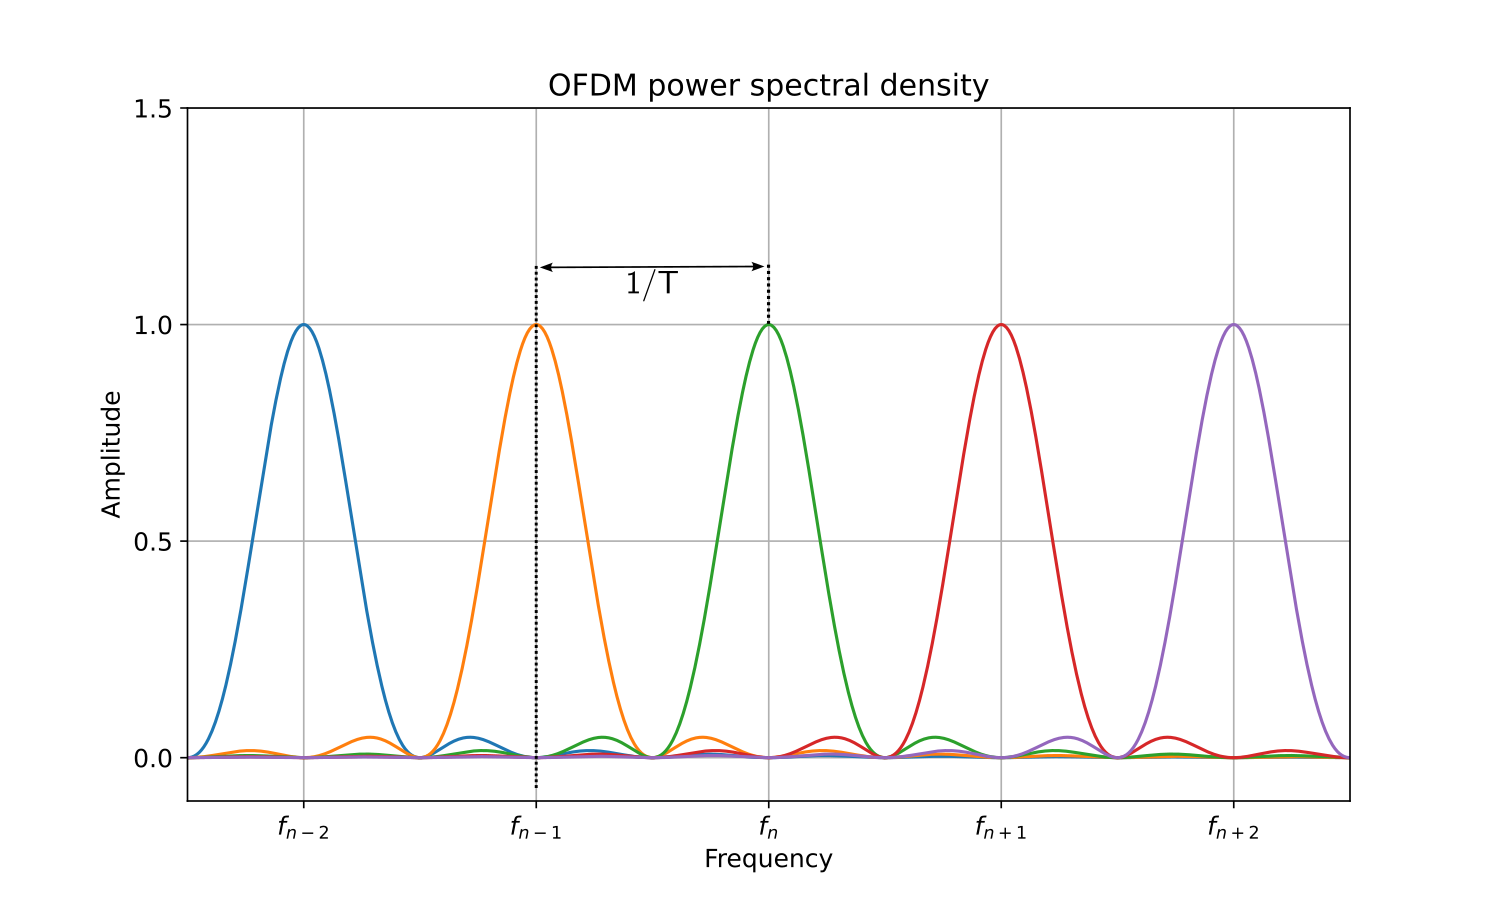
\includegraphics[width=0.7\textwidth]{images/theoretical/ofdm/ofdm_psd_mod.png}
    \caption{Example of power spectral density of an OFDM signal with N = 4.}
    \label{fig:quadtree}
\end{figure}

\subsubsection{Subcarriers and frequency spacing}
OFDM systems will use \textit{N} subcarriers, namely with frequencies $f_0$ to $f_{N-1}$, and M time-slots that will limit the temporal length of the OFDM signal.
Each set of modulated data transmitted in a single time slot will be referred as an OFDM \textit{symbol}, while the entirety NxM symbols is reffered to as an OFDM \textit{frame}.

Orthogonality of subcarriers is guaranteed by a frequency spacing $\Delta f$ of $1/T$, where $T$ is the duration of a single rectangular baseband pulse.

The time-domain signal can be expressed as

\begin{equation}
    s(t) = \sum_l\sum_{i=0}^{N-1} a_{i,l}\cdot \sqrt{\frac{1}{T}} rect \left( \frac{t-T/2 - lT}{T} \right)\exp{\left(\frac{j2\pi it}{T}\right)},
\end{equation}

where $a_{i,l}$ is the complex QAM symbol modulating the \textit{i-th} subcarrier in the \textit{l-th} symbol interval.

\subsection{Implementation}
The relation between the discrete samples of OFDM in the time and frequency domain enables a beneficial implementation.
Sampling the signal at interval $T/N$ we obtain a discrete version

\begin{equation}
    s_k = s(t)|_{t=k \frac{T}{N}} = \sqrt{\frac{1}{T}}\sum_{k=0}^{N-1} a_k \cdot e^{j2\pi ki/N}
\end{equation}

which is a discrete Fourier series DFS. When \textit{N} is a power of 2 the DFS can be implemented in an efficient way by the IFFT algorithm.

At the receiver, the time domain signal is sampled and each complex symbol is recovered by means of the FFT algorithm.

\subsection{Guard interval and cyclic prefix}
A frequency selective channel will apply a time-dispersion effect on the OFDM signal. This causes each symbol to "leak" into the adjacent ones, causing inter-symbol interference ISI.

In addition to ISI, also inter-carrier interference can be observed due to the loss of orthogonality of carriers.

To avoid this phenomenon, a guard interval is added to each OFDM symbol. Typically its duration is $T_G = T/8$ or $T_G = T/4$, and the total ODFM symbol duration then becomes $T_s = T + T_G$.

Due to the circular property of the discrete inverse Fourier transform, extending the time duration of the OFDM symbol by a guard time is equivalent to prepending a copy of the last $T_G/T$ portion of the symbol.

% TODO: insert scheme of OFDM communication

A more thorough theoretical examination of OFDM, multicarrier communications and their applications can be found in \cite{OFDMWireless} and \cite{Proakis_2001}.


\section{OFDM radar processing}
        
    During the radar operation each OFDM frame is reflected by passive targets. The received signal is a superposition of the effect of the reflection of all the targets hit by the wave front, as described in section 3.2 of \cite{Braun2014OFDMRA}, by Braun.
    
    The received signal is then
    
    \begin{equation}
    \label{eq:received_signal_mltiple_targets}
        r(t) = \sum_{h=0}^{H-1} b_h s(t-\tau_h)e^{j2\pi f_{D,h}t}e^{j\hat{\varphi}_h} + \hat{z}(t),
    \end{equation}
    
    where $s(t)$ is influenced by the factors:
    
    \begin{itemize}
        \item Magnitude attenuation factor $$b_h = \sqrt{\frac{c_0\sigma_{RCS,h}}{(4\pi)^3 d_h^4f_C^2}},$$
    that depends on the distance of the target $d_h$, its radar cross section (RCS), the speed of light $c_0$ and the carrier frequency $f_C$.
    
        \item Time delay $\tau_h = 2\frac{d_h}{c_0},$ which is the round trip time of the reflected signal.
    
        \item A Doppler shift term introduced by the relative speed of the target $f_{d,h} = 2 \frac{v_{rel,h}}{c_0}f_C$.
        \item A random phase rotation $\varphi_h$.
        \item Additive white Gaussian noise $\hat{z}(t)$.
    \end{itemize}
    
    Following Braun's notation each transmitted OFDM frame is indicated as
    \begin{equation}
        \mathbf F_{Tx} = \begin{pmatrix}
            c_{0,0} & \cdots & c_{0,M} \\
            c_{1,0} & \cdots & c_{1,M} \\
            \vdots   & \ddots & \vdots \\
            c_{N-1, 0} & \cdots & c_{N-1, M} \\
        \end{pmatrix} \in \mathcal{A}^{N\times M},
    \end{equation}
    
    where rows are different subcarriers and columns are different time slots.
    
    The received frame matrix $\mathbf F_{Rx}$ is obtained by analog/digital conversion of the signal, removal of CP from each OFDM symbol, and computing the FFT of length $N_{\text{subcarriers}}$ for every column of the matrix.
    
    \subsection{Effect of targets on OFDM frames}
    Each target reflection will influence different elements of the frame in a different way:
    
    \begin{enumerate}
        \item A Doppler frequency shift $f_D$ is equivalent to modulating the elements of each row of $F_{TX}$ by a factor $e^{j2\pi f_D T_0 l},\quad  l = 0, \cdots, M-1$.
        \item A round trip delay $\tau$ will influence each subcarrier differently, based on its frequency. The corresponding phase shift on the k-th subcarrier is $e^{-j2\pi (k\Delta f + f_0)\tau}$.
    \end{enumerate}
    
    For the single target case, H=1, the received OFDM frame will become
    
    \begin{equation}
        (\mathbf F_{Rx})_{k,l} = b_0(\mathbf F_{Tx})_{k,l} \cdot e^{j2\pi T_0 f_{D,0} l}\cdot e^{-j2\pi k \tau_0 \Delta f} \cdot e^{j\varphi_0} + (\mathbf{\Tilde{Z}})_{k,l}.
    \end{equation}
    
    The channel state information matrix (CSI) is obtained from the received frame $\mathbf{F}_{Rx}$ by removing the known transmitted frame $\mathbf{F}_{Tx}$, which serves no purpose for radar estimation. After element-wise division the CSI is
    
    \begin{equation}
        (\mathbf F)_{k,l} = \frac{(\mathbf F_{Rx})_{k,l}}{(\mathbf F_{Tx})_{k,l}} = b_0 \cdot e^{j2\pi T_0 f_{D,0} l}\cdot e^{-j2\pi k \tau_0 \Delta f} \cdot e^{j\varphi_0} + \frac{(\mathbf{\Tilde{Z}})_{k,l}}{(\mathbf F_{Tx})_{k,l}}\label{eq:CSI_frame}.    
    \end{equation}
    
    An alternative noise matrix $(\mathbf{Z})_{k,l}$ can be defined since, after division by the transmitted frame, the noise process will be white if $(\mathbf{\Tilde{Z}})$ is white.
    
    Finally, we generalize the result to H targets by reintroducing the sum from \ref{eq:received_signal_mltiple_targets}:
    
    \begin{equation}
        (\mathbf F)_{k,l} =  \sum_{h=0}^{H-1} b_h \cdot e^{j2\pi T_O f_{D,h} l}\cdot e^{-j2\pi k \tau_h \Delta f} \cdot e^{j\varphi_h} + (\mathbf{Z})_{k,l}.
    \end{equation}
    
    \subsection{Radar problem formulation}
    
    The estimation of the round-trip delay and of the Doppler shift for each target is equivalent to a spectral estimation problem. As Braun describes it: \textit{"Estimation of frequencies of a superposition of discretely sampled complex sinusoids, and their number"}.
    
    Multiple methods can be considered to solve this problem. They can be categorised as parametric, semiparametric, or nonparametric \cite{Stoica_New_Method_Parameter_Estimation}. 
    
    In the nonparametric class the most established method is the periodogram (also referred as single-frequency least-squares method), and gives optimal results for sinusoids that are well resolved.
    
    Other established methods, which are more computationally expensive in general, are MUSIC and ESPRIT, belonging to the parametric class.
    
    \subsection{Assumptions for OFDM radar systems}
    \label{sub:assumptions_ofdm_radar}
    The following assumptions simplify the design of the algorithm, as described in section 3.2.1 of \cite{Braun2014OFDMRA}.
    
    \begin{enumerate}
    	\item No other distortion other than AWGN is induced by the transmit and receive front-ends.
    	\item The CP duration is larger than the round-trip propagation time for the furthermost target.
    	\item The sub-carrier distance is at least one order of magnitude larger than the largest occurring Doppler shift.
    	
		Assumptions 2 and 3 ensure that the received matrix will not undergo de-orthogonalisation, which is necessary for element-wise division in equation \ref{eq:CSI_frame}. These conditions ensure that the OFDM symbols are not delayed more than the CP and are not shifted by a large Doppler shift. If these conditions are met, demodulation can occur correctly.
    	
    	\item The Doppler shift is the same on every sub-carrier.
    	\item The target’s distance remains constant during the transmission of one frame.
    	
    	These assumptions are approximations of the actual conditions, as they are never exactly true for non-zero Doppler shifts. However they are good approximations if the center frequency of the system is far greater then the total bandwidth and if the OFDM frames duration remains in the order of milliseconds.
    \end{enumerate}
    
    \subsection{Non ambiguous range and speed}
    
        Due to the discrete nature of $\mathbf{F}$ range and speed measurements can be estimated without ambiguity if $|T_O f_D| < 1/2$ and $\tau \Delta f < 1$ are true.
        
        From this, the unambiguous range and speed values of the system can be derived.
        
        \begin{itemize}
            \item Max unambiguous range
            $$ d_{unamb} = \frac{c_0 \tau_{unamb}}{2} = \frac{c_0}{2\Delta f}.$$
            \item Max unambiguous speed
            $$ v_{unamb} = \frac{f_{D,unamb} c_0}{2f_C} = \frac{c_0}{2f_C T_O}.$$
        \end{itemize}
        
        As long as the target range and speed fall under $d < d_{unamb}$ and $|v| < v_{unamb}$ there will be no errors due to aliasing.
        
    \subsection{Range and speed resolution}
    
        Range and speed resolution depend respectively on bandwidth and time aperture. These depend on the number of subcarriers and symbols in the OFDM frame.
        
        \begin{itemize}
            \item Range resolution
            $$ d_{res} = \frac{c_0}{2 T_S f_C N}, $$
            \item Speed resolution
            $$ v_{res} = \frac{c_0}{2\Delta_f M}. $$
        \end{itemize}
        

        
\section{Periodogram-based estimation algorithms}
    
    A periodogram is defined as the estimator of a signal's power spectral density (PSD).
    
    Considering a discrete-time signal $s(k)$ of length $N$ samples the periodogram is defined as
    
    \begin{equation}
        \text{Per}_{s(k)}(f) = \frac{1}{N}\left| \sum_{k=0}^{N-1} s(k)e^{-j2\pi fk}\right|^2.
    \end{equation}

    The optimal way to obtain the periodogram in digital systems is by quantizing the frequency at regular intervals and using the Fast Fourier Transform FFT algorithm.

    \begin{align}
        \text{Per}_{s(k)}(f) &= \frac{1}{N}\left| \sum_{k=0}^{N-1} s(k)e^{-j2\pi \frac{nk}{N_{Per}}}\right|^2 \\
        &= \frac{1}{N}\left| \text{FFT}_{N_{Per}}[s(k)]\right|^2.
    \end{align}
    
    
    The transform is indicated as $\text{FFT}_{N_{per}}$ where $N_{Per} \geq N$ is the length of the FFT. When the input signal has $N < N_{Per}$, it is zero padded to the length of the FFT.
    The transform can be calculated in the most efficient way when $N_{Per}$ is a power of 2, hence it is recommended to zero pad the input signal to the closest one.

    The input data for the periodogram is the CSI $\bm{F}$, and the periodogram is estimated in two dimensions

    \begin{align}
        \text{Per}_{\bm{F}}(n,m) &= \frac{1}{NM} \left| \underbrace{ \sum_{k=0}^{N_{Per}-1}  \overbrace{\left(  \sum_{l=0}^{M_{Per}-1} (\bm{F})_{k,l} e^{-j2\pi \frac{lm}{M_{Per}}} \right)}^{\text{N FFTs of length $M_{Per}$}}  e^{j2\pi\frac{kn}{N_{Per}}}}_{ \text{$M_{Per}$ iFFTs of length $N_{Per}$ }} \right| ^ 2 \label{eq:periodogram_full}\\
        &= \frac{1}{NM} \left| \text{CPer}_{\bm{F}}(n,m) \right| ^ 2. \label{eq:periodogram_cper}
    \end{align}


    Each target captured in the CSI, \ie a sinusoid in $\bm{F}$, results in a peak in $Per_{\bm{F}}(n,m)$.
    For each target, the frequencies of its sinusoids $\hat{\Omega}_d$ (column-wise) and $\hat{\Omega}_v$ (row-wise) in $\bm{F}$ will correspond to peaks at position $(\hat{n}, \hat{m})$ in the periodogram. Inversely, if $\text{Per}_{\bm{F}}(\hat{n},\hat{m})$ is a peak value, then the corresponding oscillation frequencies in $\bm{F}$ are $\hat{\Omega}_d = 2\pi\hat{n}/N_{\text{Per}}$ column-wise and $\hat{\Omega}_v = 2\pi\hat{m}/M_{\text{Per}}$ row-wise.
    
    These frequencies are converted into distance and relative speed as

    \begin{align}
        \hat{d} &= \frac{1}{2}\hat{\tau}c_0 = \frac{\hat{\Omega}_d c_0}{2 (2\pi) \Delta_f} = \frac{\hat{n}c_0}{2\Delta_f N_\text{Per}}, \\
        \hat{v} &= \frac{\hat{f}_D c_0 }{2 f_C} = \frac{\hat{\Omega}_v c_0}{2(2\pi)f_CT_0} =  \frac{\hat{m}c_0}{2f_cT_0 M_{\text{Per}}}.
    \end{align}
    
    % TODO: add from Braun's page 25
    
    

    As demonstrated by Braun, computing the periodogram results in a SNR gain of a factor $NM$. The numerator in \ref{eq:periodogram_full} is an accumulation of all the elements in $\bm{F}$ whereas the denominator is a superposition of complex Gaussian random variables.
    
	\subsection{Window functions}
	
	Window functions are commonly applied to signals when computing the periodogram. This operation is done to tune the sidelobe level and enable precise detection of targets. 
	
		%TODO generate image w/ and w/o windowing 
	
	The two dimensional window matrix to be applied to the periodogram $\bm{W} \in \mathbb{R}^{N\times M}$ is multiplied element-wise with the matrix $\bm{F}$. When computing the periodogram equation \ref{eq:periodogram_full} becomes
	
	
	   \begin{align}
		\text{Per}_{\bm{F}}(n,m) &= \frac{1}{NM} \left| \underbrace{ \sum_{k=0}^{N_{Per}-1}  \overbrace{\left( \sum_{l=0}^{M_{Per}-1} (\bm{F})_{k,l} (\bm{W})_{k,l} e^{-j2\pi \frac{lm}{M_{Per}}} \right)}^{\text{N FFTs of length $M_{Per}$}}  e^{j2\pi\frac{kn}{N_{Per}}}}_{ \text{$M_{Per}$ iFFTs of length $N_{Per}$ }} \right| ^ 2 \label{eq:periodogram_full_win}\\
		&= \frac{1}{NM} \left| \text{CPer}_{\bm{F}}(n,m) \right| ^ 2. \label{eq:periodogram_cper_win}
	\end{align}
	 
	 If no windowing is considered then $(\bm{W})_{k,l} = 1$, as in a simple boxcar window.
	 
	 In the proposed OFDM radar system, the following window types are of interest:
	 
	 \begin{itemize}
	 	\item Rectangular (Boxcar) windows.
	 	\item Hamming windows.
	 	\item Blackman-Harris windows.
	 	\item Dolph-Chebyshev windows.
	 \end{itemize}
	
	
	Since the width of the main lobe and the height of its peak is different from each window the windowing operation results in a SNR loss when computing the periodogram.
	The overall processing gain can be updated as
	
	\begin{align}
		PG = 10\log_{10}(NM) + \text{SNR}_{\bm{w}_d} + \text{SNR}_{\bm{w}_v},
	\end{align}
	
	where the SNR for each direction is equal to the DC bin of the periodogram of each window normalized by the width of the rectangular window.
	
	
	\subsection{Welch's method}
	
	This method, also known as window-overlap spectral analysis (WOSA), is a method of reducing the noise of the spectra estimated by calculating the periodogram, in exchange for a reduction in frequency resolution \cite{Welch_period}, \cite{Spagnolini_ch14}.
	The signal is divided into $M$ data segments of $N$ samples, the periodogram is then computed separately for each segment and then averaged.
	
	For a one-dimensional time signal \textit{x} \cite{SASPWEB2011}\footnote{\texttt{https://ccrma.stanford.edu/$\sim$jos/sasp/Welch\_s\_Method.html}}, the \textit{m}-th windowed and zero padded frame is
	
	\begin{align}
		x_m(n) = w(n)x(n + mR), \; n=0,1,\ldots, M-1, m=0,1,\ldots, K-1,
	\end{align}
	
	where R is the window's hop size and K the number of available segments. The periodogram of the \textit{m}-th block is obtained as
	
	\begin{align}
		\text{PER}_{x_m,M}(w_k) = \frac{1}{M} |\text{FFT}_{N,k}(x_m)|^2 = \frac{1}{M}\left|\sum_{n=0}^{N-1}x_m(n)e^{-j2\pi nk/N}\right|^2.
	\end{align}
	
	The Welch estimate of the PSD is then given by
	
	\begin{align}
		\hat{S}^W_x(w_k) = \frac{1}{K}\sum_{m=0}^{K-1}\text{PER}_{x_m,M}(w_k).
	\end{align}
	
	The overall data can be windowed before computing the periodogram, reducing sidelobe level in the spectral estimate, at the expense of frequency resolution. If $w(n)$ is a rectangular window then the periodograms are formed from non-overlapping successive blocks of data (we can refer to this case as Barlett's method). For different kinds of windows the hop size $R$ shouldn't exceed half of the frame length $M/2$. In general $R$ is chosen so that consecutive windows overlap and add to a constant.
	
	
	

	

    
    
    